\chapter{Evaluation}
\label{chapter:Evaluation}
We evaluated our tool X with Y popular servers, by instrumenting them with our tool.
We performed runtime performance test with the following applications.

Our Evaluation aims to answer the following research questions:
\begin{itemize}
 \item \textbf{R1:} How efective is out tool in securing binary programs against the COOP attack?
 
 \item \textbf{R2:} How precise is our tool in detecting the types of the caller/caller pairs?
 
 \item \textbf{R3:} What is the performance overhead of our tool?
 
 \item \textbf{R4:} What are the instumentation overheads imposed by our tool 
 
 \item \textbf{R5:} How many caller/called pairs are secured by our tool and how many remain unsecured?
 
 \item \textbf{R6:} Against which kind of attacks can our tool secure programs?
 
 \item \textbf{R7:} What are the Limitations of our Tool?
 
 \item \textbf{R8:} List is not exauhustive. Give another relevant research question. if there is one.
 
\end{itemize}

\textbf{Comparison methods.} Example: We used UBSAN (compare with TypeArmor), the state-of-art
tool for detecting bad-casting bugs, as our comparison tar-
get of C A V ER . Also, We used C A V ER - NAIVE , which dis-
abled the two optimization techniques described in §4.4,
to show their effectiveness on runtime performance opti-
mization.

\textbf{Experimental setup.} Example: All experiments were run on
Ubuntu 13.10 (Linux Kernel 3.11) with a quad-core 3.40
GHz CPU (Intel Xeon E3-1245), 16 GB RAM, and 1 TB
SSD-based storage.


\section{R1: Effectiveness of our Tool}
\begin{table}[H]
\centering
\caption{Classification CS}
\label{Integer overflow bug detection in CWE-190}
\resizebox{.99\columnwidth}{!}{%
\begin{tabular}{|l|l|l|l|l|l|l|l|l|l|l|l|l|} \hline
\textbf{target}  &\textbf{opt} & \textbf{\#CS}     & \textbf{problems}    &\textbf{0} & \textbf{-1}  & \textbf{-2} &\textbf{-3} &\textbf{-4} &\textbf{-5} &\textbf{-6}  &\textbf{non-void-ok}  &\textbf{non-void-probl.}   \\ \hline 
x                &x            &x                  &x                     &x          &x             &x            &x           &x           &x           &x            &x                     &x                          \\ \hline

\end{tabular}}
%  \vspace{-2.5em}
\end{table}


\begin{table}[H]
\centering
\caption{Compound}
\label{Integer overflow bug detection in CWE-190}
\resizebox{.99\columnwidth}{!}{%
\begin{tabular}{|l|l|l|l|l|l|l|l|l|l|l|l|} \hline
\textbf{opt}  & \textbf{\#CS}     & \textbf{cs args (perfect \%)}    &\textbf{cs args (problem \%)} & \textbf{cs non-void (correct \%)}  & \textbf{cs non-void (probl. \%)} &\textbf{\#ct} &\textbf{ct args (perfect \%)} &\textbf{ct args (probl. \%)} &\textbf{ct void (correct \%)}  &\textbf{ct void (correct \%)}   \\ \hline 
x             &x                  &x                                 &x                             &x                                   &x                                 &x             &x                             &x                            &x                              &x                               \\ \hline

\end{tabular}}
%  \vspace{-2.5em}
\end{table}

\begin{table}[H]
\centering
\caption{Classification CT}
\label{Integer overflow bug detection in CWE-190}
% \resizebox{.99\columnwidth}{!}{%
\begin{tabular}{|l|l|l|l|l|l|l|l|l|l|l|l|l|} \hline
\textbf{target}  &\textbf{opt} & \textbf{\#CS}     & \textbf{problems}    &\textbf{0} & \textbf{-1}  & \textbf{-2} &\textbf{-3} &\textbf{-4} &\textbf{-5} &\textbf{-6}  &\textbf{non-void-ok}  &\textbf{non-void-probl.}   \\ \hline 
x                &x            &x                  &x                     &x          &x             &x            &x           &x           &x           &x            &x                     &x                          \\ \hline

\end{tabular}
% }
%  \vspace{-2.5em}
\end{table}


\begin{table}[H]
\centering
\caption{Callsite Classification for paramcount}
\label{Integer overflow bug detection in CWE-190}
% \resizebox{.99\columnwidth}{!}{%
\begin{tabular}{|l|l|l|l|l|l|l|l|l|l|} \hline
\textbf{target}  & \textbf{opt}     & \textbf{problematic}    &\textbf{+0} & \textbf{+1}  & \textbf{+2} &\textbf{+3} &\textbf{+4} &\textbf{+5} &\textbf{+6}  \\ \hline 
x                &x                 &x                        &x           &x             &x            &x           &x           &x           &x            \\ \hline

\end{tabular}
% }
%  \vspace{-2.5em}
\end{table}

\begin{table}[H]
\centering
\caption{Calltarget Classification}
\label{Integer overflow bug detection in CWE-190}
% \resizebox{.99\columnwidth}{!}{%
\begin{tabular}{|l|l|l|l|l|l|l|l|l|l|} \hline
\textbf{target}  & \textbf{opt}     & \textbf{problematic}    &\textbf{-0} & \textbf{-1}  & \textbf{-2} &\textbf{-3} &\textbf{-4} &\textbf{-5} &\textbf{-6}  \\ \hline 
x                &x                 &x                        &x           &x             &x            &x           &x           &x           &x            \\ \hline

\end{tabular}
% }
%  \vspace{-2.5em}
\end{table}

\begin{table}[H]
\centering
\caption{Coumpound table}
\label{Integer overflow bug detection in CWE-190}
% \resizebox{.99\columnwidth}{!}{%
\begin{tabular}{|l|l|l|l|l|l|} \hline
\textbf{target}  & \textbf{opt}     & \textbf{\#}    &\textbf{Callsites: param perf. \%, probl \%} & \textbf{\#}  & \textbf{Callsites: param perf. \%, probl \%}  \\ \hline 
x                &x                 &x               &x                                      &x             &x                                        \\ \hline

\end{tabular}
% }
%  \vspace{-2.5em}
\end{table}


\begin{table}[H]
\centering
\caption{MAtching table}
\label{Integer overflow bug detection in CWE-190}
% \resizebox{.99\columnwidth}{!}{%
\begin{tabular}{|l|l|l|l|l|l|l|l|l|} \hline
\textbf{target}  & \textbf{opt}     & \textbf{ct}    &\textbf{Ct probl.} & \textbf{at}  & \textbf{at prob.} &\textbf{cs} & \textbf{clang cs probl.}  & \textbf{padyn cs probl.}  \\ \hline 
x                &x                 &x               &x                  &x             &x                  &x           &x                          &x   \\ \hline

\end{tabular}
% }
%  \vspace{-2.5em}
\end{table}


\begin{table}[H]
\centering
\caption{policy evaluation}
\label{Integer overflow bug detection in CWE-190}
% \resizebox{.99\columnwidth}{!}{%
\begin{tabular}{|l|l|l|l|l|l|l|l|l|l|l|} \hline
\textbf{target}  & \textbf{opt}     & \textbf{policy}    &\textbf{0} & \textbf{1}  & \textbf{2} &\textbf{3} & \textbf{4}  & \textbf{5} & \textbf{6}  & \textbf{sumarry}  \\ \hline 
x                &x                 &x                   &x          &x            &x           &x          &x            &x           &x            &x \\ \hline

\end{tabular}
% }
%  \vspace{-2.5em}
\end{table}

\begin{table}[H]
\centering
\caption{param wideness}
\label{Integer overflow bug detection in CWE-190}
% \resizebox{.99\columnwidth}{!}{%
\begin{tabular}{|l|l|l|l|l|l|l|} \hline
\textbf{5}  & \textbf{4}     & \textbf{3}    &\textbf{2} & \textbf{1}  & \textbf{0} &\textbf{param/wideness}  \\ \hline 
x           &x               &x              &x          &x            &x           &0                         \\ \hline
x           &x               &x              &x          &x            &x           &8                         \\ \hline
x           &x               &x              &x          &x            &x           &16                         \\ \hline
x           &x               &x              &x          &x            &x           &32                         \\ \hline
x           &x               &x              &x          &x            &x           &64                         \\ \hline

\end{tabular}
% }
%  \vspace{-2.5em}
\end{table}

\begin{table}[H]
\centering
\caption{tabelle 7}
\label{Integer overflow bug detection in CWE-190}
% \resizebox{.99\columnwidth}{!}{%
\begin{tabular}{|l|l|l|l|l|l|l|} \hline
\textbf{5}  & \textbf{4}     & \textbf{3}    &\textbf{2} & \textbf{1}  & \textbf{0} &\textbf{param/wideness}  \\ \hline 
x           &x               &x              &x          &x            &x           &0                         \\ \hline
x           &x               &x              &x          &x            &x           &8                         \\ \hline
x           &x               &x              &x          &x            &x           &16                         \\ \hline
x           &x               &x              &x          &x            &x           &32                         \\ \hline
x           &x               &x              &x          &x            &x           &64                         \\ \hline

\end{tabular}
% }
%  \vspace{-2.5em}
\end{table}

\begin{table}[H]
\centering
\caption{tabelle 7}
\label{Integer overflow bug detection in CWE-190}
% \resizebox{.99\columnwidth}{!}{%
\begin{tabular}{|l|l|l|l|l|l|l|} \hline
\textbf{5}  & \textbf{4}     & \textbf{3}    &\textbf{2} & \textbf{1}  & \textbf{0} &\textbf{param/wideness}  \\ \hline 
x           &x               &x              &x          &x            &x           &0                         \\ \hline
x           &x               &x              &x          &x            &x           &8                         \\ \hline
x           &x               &x              &x          &x            &x           &16                         \\ \hline
x           &x               &x              &x          &x            &x           &32                         \\ \hline
x           &x               &x              &x          &x            &x           &64                         \\ \hline

\end{tabular}
% }
%  \vspace{-2.5em}
\end{table}

% http://www.texample.net/tikz/examples/
% 
% \begin{tikzpicture}[node distance=1cm, auto,]
%  %nodes
%  \node[punkt] (market) {Market (b)};
%  \node[punkt, inner sep=5pt,below=0.5cm of market]
%  (formidler) {Intermediaries (c)};
%  % We make a dummy figure to make everything look nice.
%  \node[above=of market] (dummy) {};
%  \node[right=of dummy] (t) {Ultimate borrower}
%    edge[pil,bend left=45] (market.east) % edges are used to connect two nodes
%    edge[pil, bend left=45] (formidler.east); % .east since we want
%                                              % consistent style
%  \node[left=of dummy] (g) {Ultimate lender}
%    edge[pil, bend right=45] (market.west)
%    edge[pil, bend right=45] (formidler.west)
%    edge[pil,<->, bend left=45] node[auto] {Direct (a)} (t);
% \end{tikzpicture}
% \vspace{1em}
% \emph{Impact of CFi and CFC example.}

alternative for abobe:
\begin{figure}[!ht]
  \caption{impact of CFI and CFC}
  \centering
    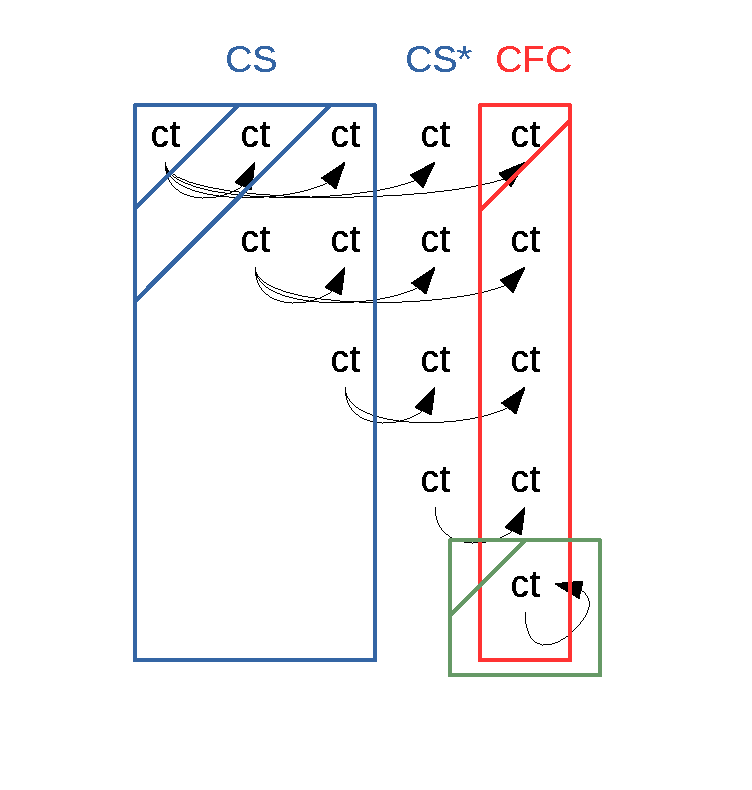
\includegraphics[width=0.5\textwidth]{figures/impact_of_cfi_and_cfc.pdf}
\end{figure}

\begin{figure}[!ht]
  \caption{liveness iteration, dummy}
  \centering
    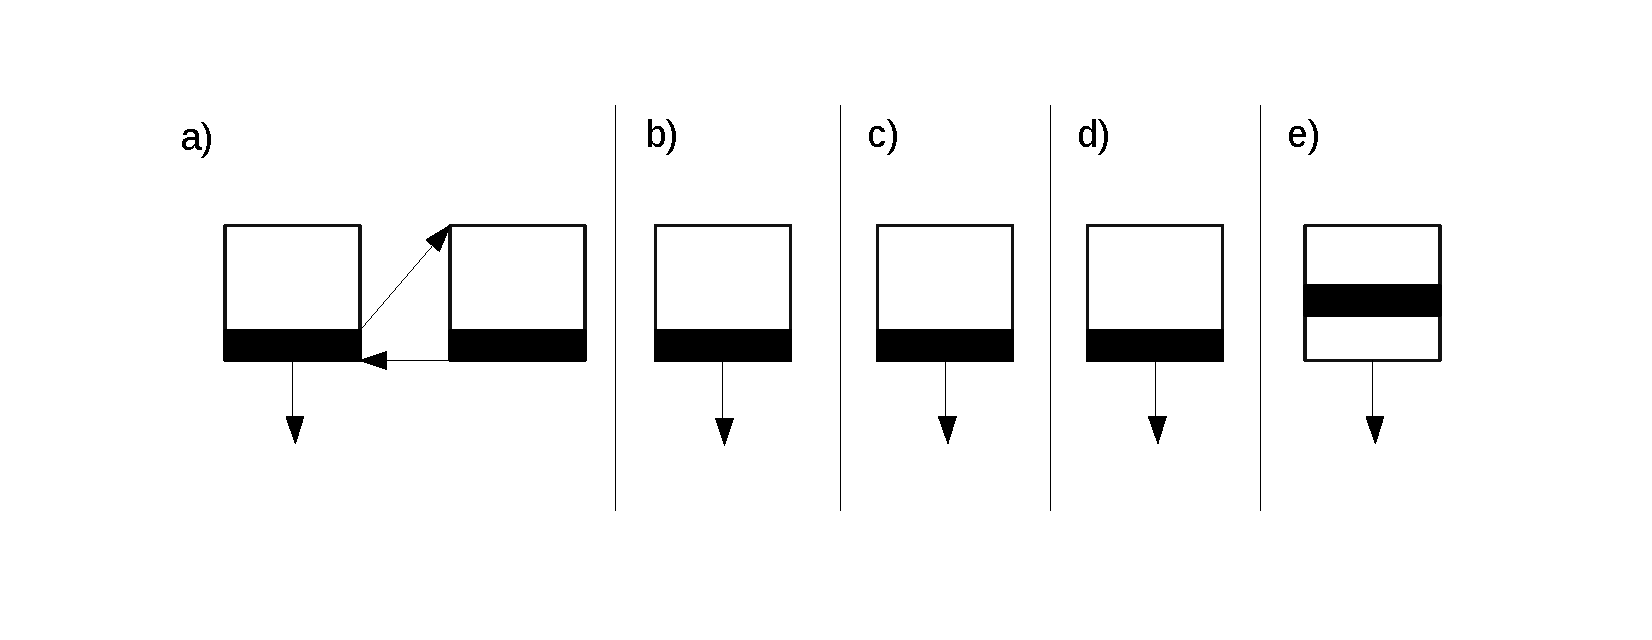
\includegraphics[width=0.9\textwidth]{figures/liveness_iteration.pdf}
\end{figure}

\begin{figure}[!ht]
  \caption{reaching iteration, dummy}
  \centering
    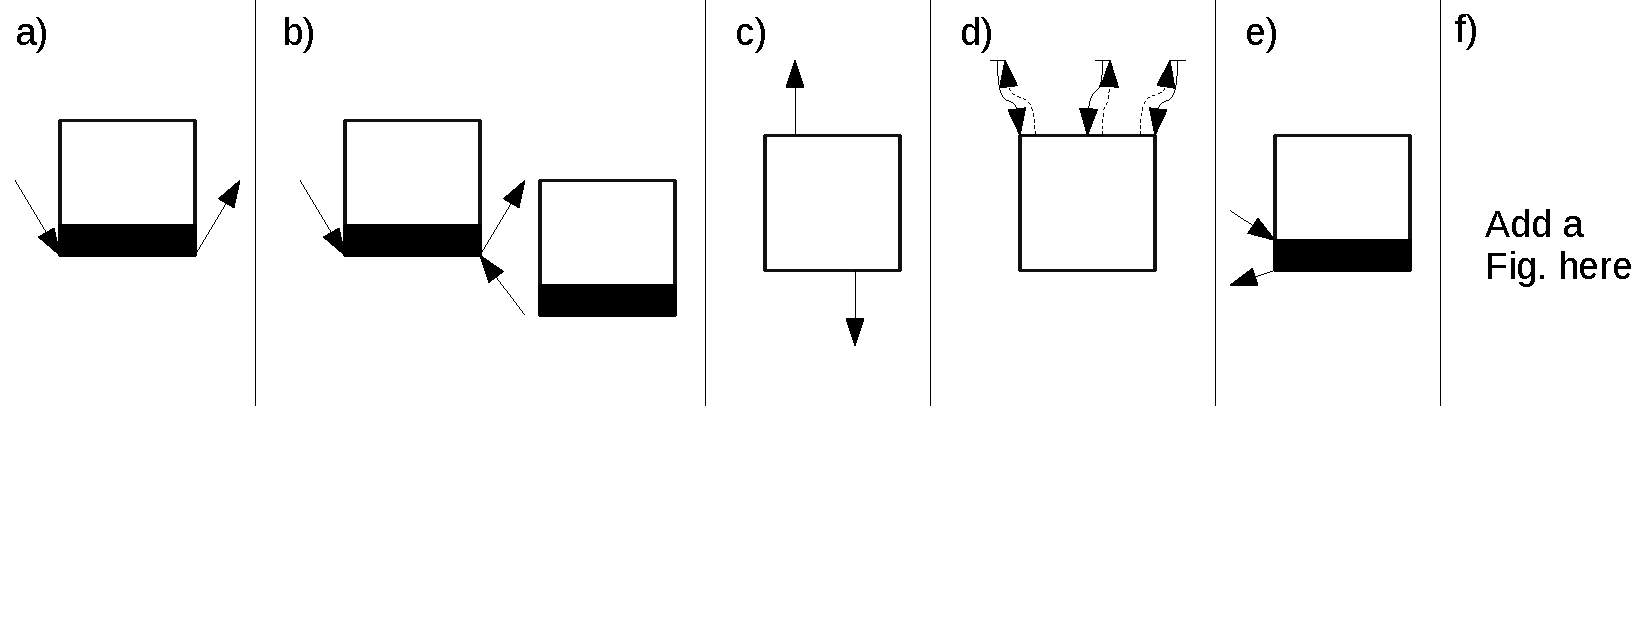
\includegraphics[width=0.9\textwidth]{figures/reaching_iteration.pdf}
\end{figure}





\begin{table}[H]
\centering
\caption{matching}
\label{matching}
\resizebox{.99\columnwidth}{!}{%
\begin{tabular}{|l|l|l|l|l|l|l|l|l|} \hline
\textbf{target}  & \textbf{opt}     & \textbf{fn\_count}    &\textbf{fn\_problem} & \textbf{at\_count}  & \textbf{at\_problem} &\textbf{cs\_count} & \textbf{cs\_clang} &\textbf{cs\_padyn} \\ \hline 
x                &x                 &x                      &x                    &x                    &x                     &0                  &0                   &0                  \\ \hline


\end{tabular}
}
%  \vspace{-2.5em}
\end{table}

\begin{table}[H]
\centering
\caption{pairings compares}
\label{matching}
% \resizebox{.99\columnwidth}{!}{%
\begin{tabular}{|l|l|l|l|l|l|l|l|l|l|l|} \hline
\textbf{target}  & \textbf{opt}     & \textbf{policy} & \textbf{0}    &\textbf{1} & \textbf{2}  & \textbf{3} &\textbf{4} & \textbf{5} &\textbf{6}  &\textbf{summary} \\ \hline 
proftpd          &x                 &x                &x              &x          &x            &0           &0          &0           &0           &0     \\ \hline
proftpd          &x                 &x                &x              &x          &x            &0           &0          &0           &0           &0      \\ \hline
vsftpd           &x                 &x                &x              &x          &x            &0           &0          &0           &0           &0      \\ \hline
vsftpd           &x                 &x                &x              &x          &x            &0           &0          &0           &0           &0      \\ \hline

\end{tabular}
% }
%  \vspace{-2.5em}
\end{table}

\begin{table}[H]
\centering
\caption{policy baseline}
\label{matching}
% \resizebox{.99\columnwidth}{!}{%
\begin{tabular}{|l|l|l|l|l|l|l|l|l|l|l|} \hline
\textbf{target}  & \textbf{opt}     & \textbf{policy} & \textbf{0}    &\textbf{1} & \textbf{2}  & \textbf{3} &\textbf{4} & \textbf{5} &\textbf{6}  &\textbf{summary} \\ \hline 
proftpd          &x                 &x                &x              &x          &x            &0           &0          &0           &0           &0     \\ \hline
proftpd          &x                 &x                &x              &x          &x            &0           &0          &0           &0           &0      \\ \hline
vsftpd           &x                 &x                &x              &x          &x            &0           &0          &0           &0           &0      \\ \hline
vsftpd           &x                 &x                &x              &x          &x            &0           &0          &0           &0           &0      \\ \hline

\end{tabular}
% }
%  \vspace{-2.5em}
\end{table}


\section{R2: Precision of our Tool}

\section{R3: Performance overhead of our Tool}

\section{R4: Instrumentation overhead of our Tool}

\section{R5: Security coverage of our tool}

\section{R6: Which kind of attacks can our tool defend off}

\section{R7: Whar are the limitations of our Tool}

\section{R8: To Do.}


it is easier for the reader if we can directly map those section from underneath on the section from above.

\section{Classification}
\subsection{Callsites}
overestimation param count. table.
number of parameters.

\subsection{Calltargets}
underestimation param table.

\section{Patching Policies}
Two types of diagrams. Table 5 from TypeArmor and a CDF to compare param count and param type. (baseline).
\subsection{AT}
\subsection{ParamCount}
table, cdf, baseline vs. server. approximations.

\subsection{ParamType}
table, cdf, baseline vs. server. approximations.

\section{Security Evaluation}

\section{Performance}
spec 2006.